%!TEX root = ../document.tex
\chapter{ARP Spoofing}
\label{chapter_arp_spoofing}
ARP Spoofing ist ein Man-In-The-Middle-Angriff (MITM-Angriff) mit dem Ziel, den Netzwerkverkehr von einem oder mehreren fremden Rechnern zu überwachen und zu manipulieren.

\section{Erklärung}
Für die Kommunikation über ein Netzwerk wird die MAC-Adresse des Zielrechners genutzt. Da meist nur die IP-Adresse zur Verfügung steht, gibt es das Address Resolution Protocol (ARP), mit dessen Hilfe eine Verknüpfung zwischen den beiden Adressen hergestellt werden kann. Außerdem hat jeder Rechner eine ARP-Tabelle in der sämtliche bekannte Verknüpfungen zwischen IP- und ARP-Adresse gespeichert werden. In Abbildung \ref{fig:arp_tabelle_vorher} wird eine unveränderte ARP-Tabelle dargestellt. Es ist in jeder Zeile eine IP-Adresse mit der zugehörigen MAC-Adresse (physische Adresse), sowie deren Typ zu sehen. Der Typ kann dabei statisch -- und damit nachträglich nicht mehr veränderbar -- oder dynamisch sein.

\begin{figure}
	\centering
	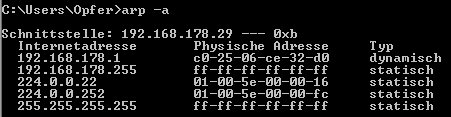
\includegraphics[width=\textwidth]{images/arp/ARP_Tabelle_Vorher}
	\caption{Unveränderte ARP-Tabelle mit dynamischen und statischen Einträgen}
	\label{fig:arp_tabelle_vorher}
\end{figure}

Möchte nun ein Rechner Daten versenden, so wird als erstes in der eigenen ARP-Tabelle nach dem Zielrechner gesucht. Existiert noch kein Eintrag, verschickt der Rechner einen ARP-Request an die Broadcast-MAC-Adresse, um die MAC-Adresse zu seiner Ziel-IP-Adresse von den anderen Netzwerkteilnehmern zu erfragen. Abbildung \ref{fig:arp_request} zeigt einen möglichen Aufbau eines solchen ARP-Requests. Daraufhin schickt der Zielrechner seine MAC-Adresse mittels eines ARP-Replys direkt an den Quellrechner zurück. Ein beispielhafter Aufbau eines ARP-Replys ist in Abbildung \ref{fig:arp_reply} dargestellt. Der Quellrechner legt für diese Verknüpfung einen neuen Eintrag in seiner ARP-Tabelle an und kann daraufhin die Daten versenden.

\begin{figure}
	\centering
	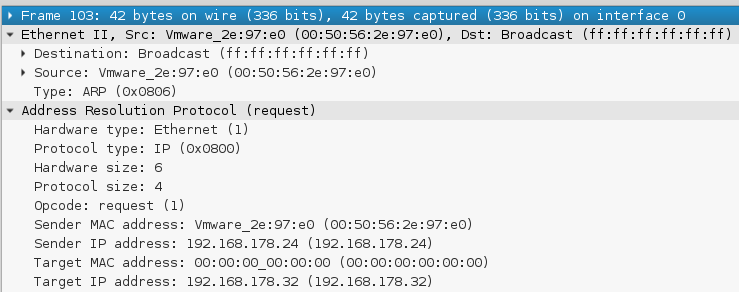
\includegraphics[width=\textwidth]{images/arp/ARP_Request}
	\caption{Aufgezeichneter ARP-Request für die Adresse 192.168.178.32 mit leerer MAC-Adresse}
	\label{fig:arp_request}
\end{figure}

\begin{figure}
	\centering
	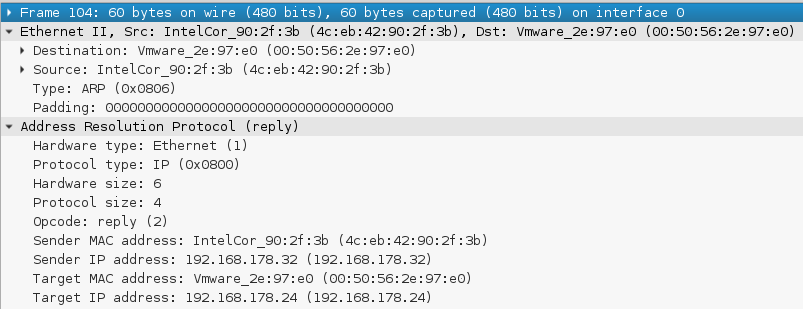
\includegraphics[width=\textwidth]{images/arp/ARP_Reply}
	\caption{Aufgezeichneter ARP-Reply von der Adresse 192.168.178.32 mit der zugehörigen MAC-Adresse}
	\label{fig:arp_reply}
\end{figure}

Da im Jahr 1982 bei Erscheinen des Protokolls nur dessen Funktionalität und nicht dessen Sicherheit relevant war, wurden die Schwächen des Protokolls erst im Nachhinein entdeckt. So wird bei einem eingehenden ARP-Reply nicht geprüft, ob es zuvor einen ARP-Request gab. Es wird also lediglich ein Eintrag in der ARP-Tabelle generiert oder ein bestehender Eintrag geändert.

Dies kann sich ein Angreifer zu Nutze machen und sämtliche IP-Adressen mit seiner eigenen MAC-Adresse verknüpfen. Ein solcher manipulierter ARP-Reply ist in Abbildung \ref{fig:arp_fake_reply} dargestellt. Nach diesem ARP-Reply bekommt der Angreifer alle versendeten Daten und kann diese weiterleiten oder verändern. Ein Vergleich der Netzwerkkommunikation vor und nach der Manipulation der ARP-Tabelle ist in Abbildung \ref{fig:netzwerkverkehr_vergleich} skizziert.

\begin{figure}
	\centering
	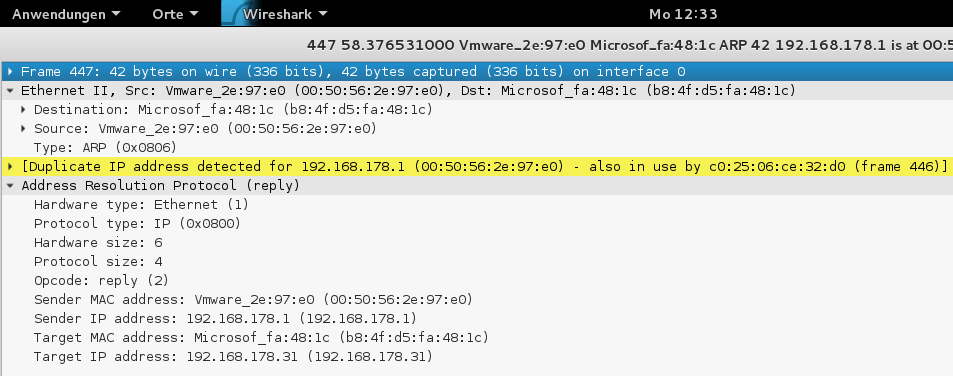
\includegraphics[width=\textwidth]{images/arp/ARP_Fake_Reply}
	\caption{Manipulierter ARP-Reply der beim Zielrechner die IP-Adresse eines dritten Rechners mit der MAC-Adresse des Angreifers verknüpft}
	\label{fig:arp_fake_reply}
\end{figure}

\begin{figure}
	\centering
	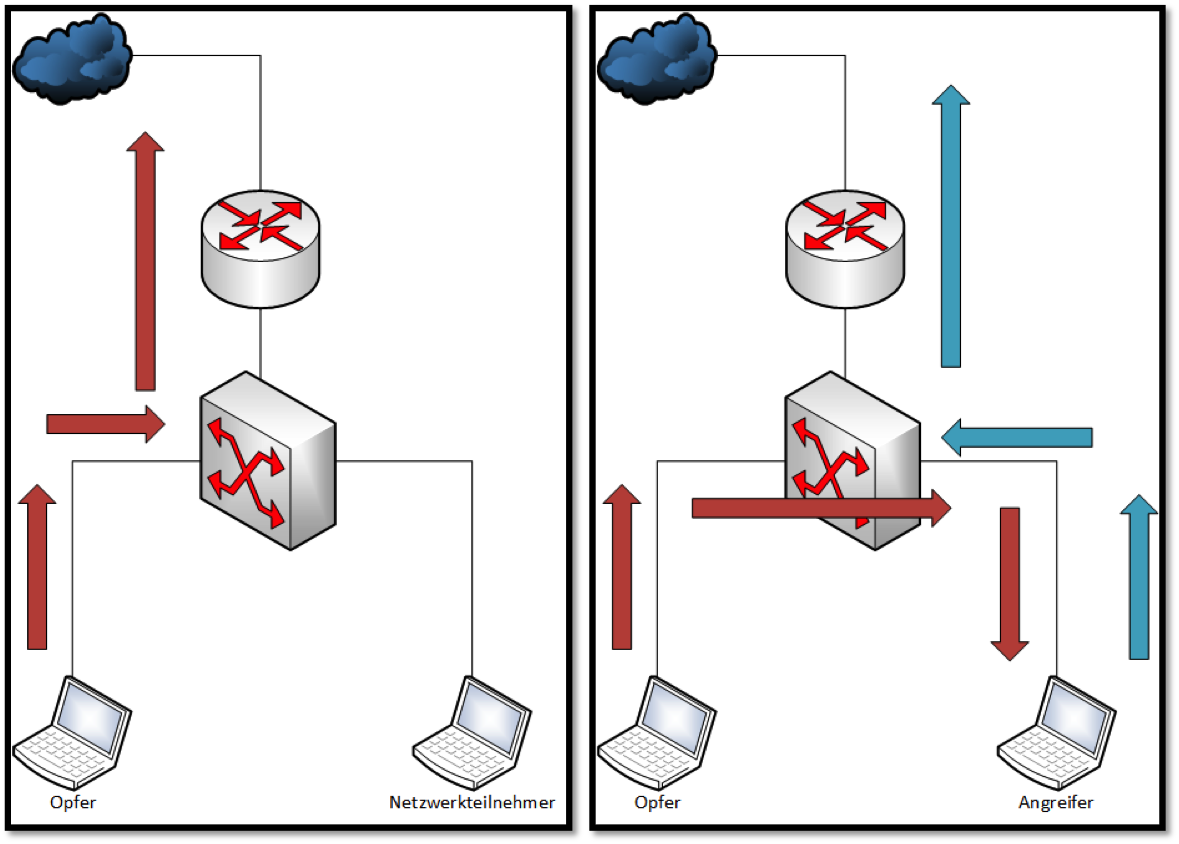
\includegraphics[width=\textwidth]{images/arp/Netzwerkverkehr_Vergleich}
	\caption{links: Netzwerkkommunikation über das Gateway des Netzes direkt mit anderen Netzwerkteilnehmern; rechts: Netzwerkkommunikation erfolgt immer über den Rechner des Angreifers}
	\label{fig:netzwerkverkehr_vergleich}
\end{figure}

\section{Vorbereitung}
Notwendige Hardware:

\begin{itemize}
	\item Kali Linux 2.0 mit der Security Workbench (Rechner des Angreifers)
	\item Kali Linux 2.0 mit der Security Workbench (Rechner des Opfers)
	\item Raspbery Pi mit Raspbian
\end{itemize}

\section{Ablauf}
Für das ARP Spoofing sind zwei unterschiedliche Tutorials vorhanden. Das erste Tutorial ist als Einstieg gedacht und beschreibt das Verändern der ARP-Tabelle an einem fremden Gerät. Das zweite Tutorial baut darauf auf und verändert dann die vom fremden Gerät aufgerufenen Homepages indem HTML-Code eingebunden wird.

Da es bei dieser Art von Attacke immer mindestens zwei Teilnehmer gibt, wird dies auch im Tutorial widergespiegelt. Es gibt die beiden Rollen \emph{Angreifer} und \emph{Opfer}, die für ein Gelingen der Attacke abwechselnd beschrieben werden.


\subsection{Darstellung des Netzwerkverkehrs}
\paragraph{Angreifer \& Opfer} Starte die Security Workbench, falls noch nicht geschehen (siehe \ref{ch:startWorkbench}: Einführung in das Arbeiten mit Linux). Der Startbildschirm ist in Abbildung \ref{fig:scriptstart} zu sehen. Wähle dort die Nummer 3 \enquote{ARP Spoofing Tutorials}

\begin{figure}
	\centering
	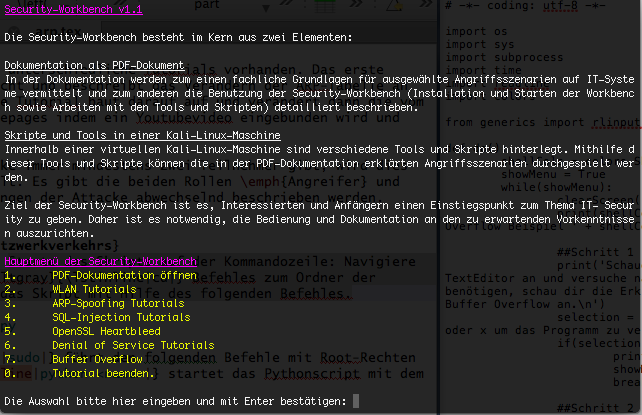
\includegraphics[width=\textwidth]{images/arp/Scriptstart}
	\caption{Bildschirmausgabe beim Start des Security Workbench Skriptes auf der Konsole}
	\label{fig:scriptstart}
\end{figure}

\paragraph{Angreifer} Wähle Nummer 1 \enquote{Einfaches ARP-Spoofing als Angreifer}

\paragraph{Opfer} Wähle Nummer 2 \enquote{Starte Darstellung des Netzwerkverkehrs als Opfer}

%\paragraph{Angreifer \& Opfer} Stelle sicher, dass du direkten Zugriff auf das Host-Netzwerk hast. Wie das geht kannst du in der PDF-Dokumentation im Kapitel \enquote{Tunneln von Netzwerkadaptern} nachlesen.

\paragraph{Opfer} Rufe die Konfiguration deiner IP-Netzwerkschnittstellen auf und lese dort deine IP-Adresse aus, um sie dem Angreifer zu sagen:
\begin{lstlisting}
ifconfig
\end{lstlisting}

\paragraph{Opfer} Rufe deine ARP-Tabelle, wie in Abbildung \ref{fig:netzwerkverkehropfer} zu sehen, mit folgendem Befehl auf.
\begin{lstlisting}
arp -a
\end{lstlisting}
(\colorbox{altgray}{\lstinline|arp|} ist ein Paket zum Anzeigen und Manipulieren des Adress Resolution Protocols, \colorbox{altgray}{\lstinline|-a|} zeigt alle aktuellen Einträge der ARP-Tabelle)

\paragraph{Angreifer} Rufe die Konfiguration deiner IP-Netzwerkschnittstellen auf und lese dort dein Netzwerkinterface aus:
\begin{lstlisting}
ifconfig
\end{lstlisting}

\paragraph{Angreifer} Gib zunächst das verwendete Netzwerkinterface deines Rechners an (in der Regel eth0 bzw. wlan0) und führe mit folgendem Befehlen einen lokalen Netzwerk-Scan durch, um die IP-Adresse des Opfers herauszufinden. Wie in Abbildung \ref{fig:arpscan} zu sehen ist, werden nun die verfügbaren IP-Adressen des Netzwerks in einer Liste dargestellt.
\begin{lstlisting}
arp-scan --interface eth0 --localnet
\end{lstlisting}
(\colorbox{altgray}{\lstinline|--interface eth0 |} benennt das zu verwendende Netzwerkinterface über das gescannt werden soll; \colorbox{altgray}{\lstinline|--localnet |} generiert die IP-Adressen mithilfe der Konfiguration des Netzwerkinterfaces)

\begin{figure}
	\centering
	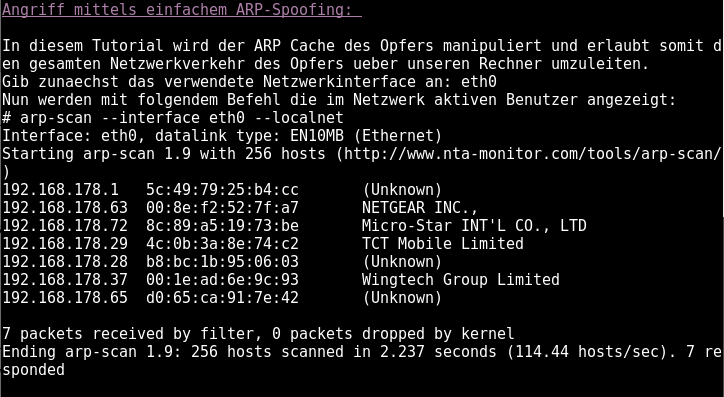
\includegraphics[width=\textwidth]{images/arp/arp_scan}
	\caption{Stand des Tutorials nachdem der ARP-Scan durchfegührt wurde}
	\label{fig:arpscan}
\end{figure}

\paragraph{Angreifer} Gib nun die IP-Adresse des gewünschten Opfers ein und starte ein ARP-Spoofing Angriff mit Ettercap.
\begin{lstlisting}
ettercap -T -i eth0 -M ARP /192.168.178.65// ///
\end{lstlisting}

\begin{itemize}
	\item \bashCommand{-T} sagt Ettercap, dass es  Informationen nur als Text darstellen und keine GUI verwenden soll
	\item \bashCommand{-i eth0} gibt das Interface an, das verwendet werden soll
	\item \bashCommand{-M ARP /192.168.178.65// ///} benennt die Art des Angriffs und das Ziel, in diesem Fall soll ein Man-in-the-Middle Angriff mithilfe von ARP-Spoofing ausgeführt werden
\end{itemize}


Ettercap zeigt uns nun in einer neuen Konsole den Netzwerkverkehr des Opfers wie in Abbildung \ref{fig:ettercaparp} beispielhaft zu sehen ist. Wichtig ist, dass die ersten Requests eingegangen sind, bevor du weitermachst.

\begin{figure}
	\centering
	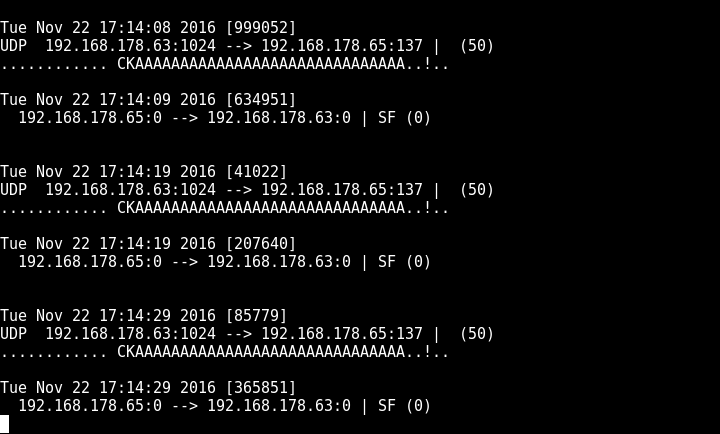
\includegraphics[width=\textwidth]{images/arp/ettercaparp}
	\caption{Ettercap zeigt den Netzwerkverkehr des Opfers an}
	\label{fig:ettercaparp}
\end{figure}

\paragraph{Opfer} Rufe noch einmal deine ARP-Tabelle, wie in Abbildung \ref{fig:netzwerkverkehropfer} zu sehen, mit folgendem Befehl auf: \colorbox{altgray}{\lstinline|arp -a|}

Beim Vergleichen der beiden Tabellen sollte auffallen, dass die dynamischen Einträge bei der zweiten Tabelle alle auf die gleiche MAC-Adresse -- die des Angreifers -- zeigen.

 \begin{figure}
	\centering
	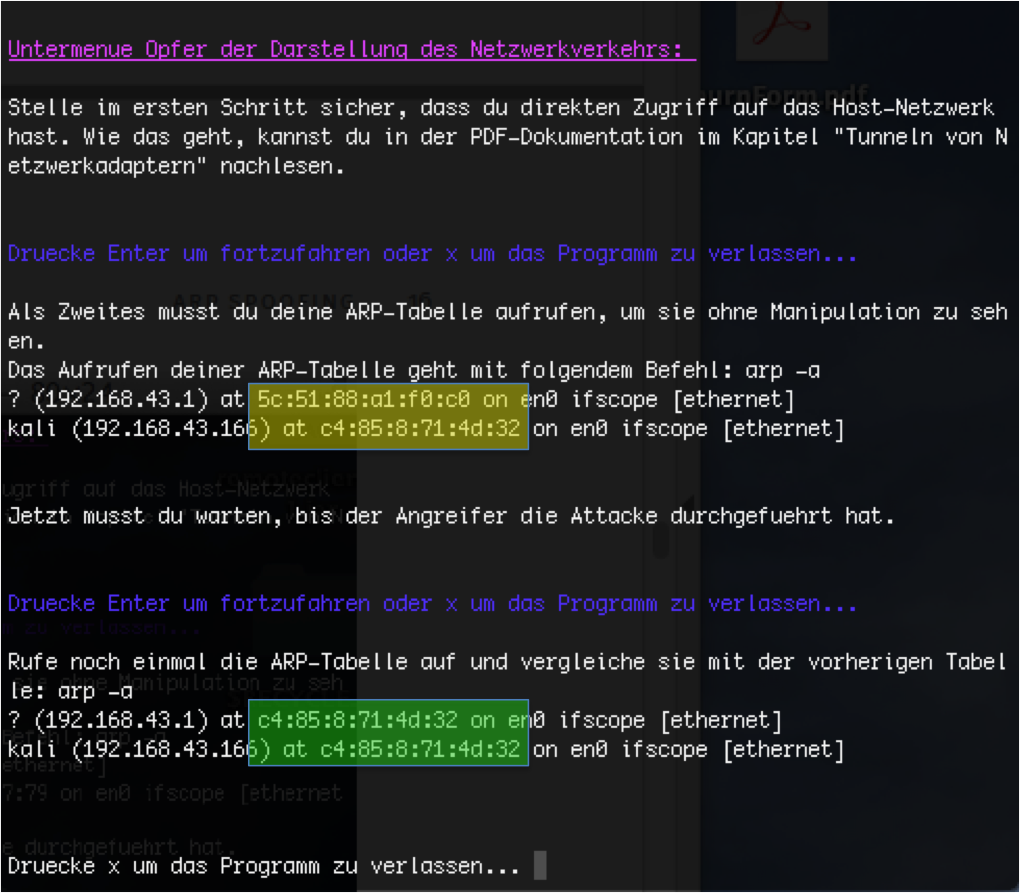
\includegraphics[width=\textwidth]{images/arp/NetzwerkverkehrOpfer}
	\caption{Ablauf des Tutorials aus Sicht des Opfers mit in gelb markierter ARP Tabelle vor dem Angriff und in grün markierter ARP Tabelle nach dem Angriff}
	\label{fig:netzwerkverkehropfer}
\end{figure}

\paragraph{Angreifer} Beende nun Ettercap durch drücken von \bashCommand{q}. Dadurch wird die ursprüngliche ARP-Tabelle des Opfers wiederhergestellt.

\subsection{Manipulation der Webseiten}
\paragraph{Angreifer \& Opfer} Starte die Security Workbench, falls noch nicht geschehen (siehe \ref{ch:startWorkbench}: Einführung in das Arbeiten mit Linux). Der Startbildschirm ist in Abbildung \ref{fig:scriptstart} zu sehen. Wähle dort die Nummer 3 \enquote{ARP Spoofing Tutorials}

\paragraph{Angreifer} Wähle Nummer 3 \enquote{ARP-Spoofing und Verwendung von Filtern}

\paragraph{Opfer} Wähle Nummer 4 \enquote{Starte Manipulation der Webseiten als Opfer}

%\paragraph{Angreifer \& Opfer} Stelle sicher, dass du direkten Zugriff auf das Host-Netzwerk hast. Wie das geht kannst du in der PDF-Dokumentation im Kapitel \enquote{Tunneln von Netzwerkadaptern} nachlesen.

\paragraph{Opfer} Rufe die Webseite news.local auf. Schließe im Anschluss den Browser.

\paragraph{Angreifer} Gib zunächst das verwendete Netwzwerkinterface deines Rechners an (in der Regel eth0 bzw. wlan0) und führe mit folgendem Befehln einen lokalen Netzwerkscan durch, um die IP-Adresse des Opfers herauszufinden. Wie in Abbildung \ref{fig:arpscan} zu sehen ist, werden nun die verfügbaren IP-Adressen des Netzwerks in einer Liste dargestellt.
\begin{lstlisting}
arp-scan --interface eth0 --localnet
\end{lstlisting}

\begin{itemize}
	\item \bashCommand{--interface eth0} benennt das zu verwendende Netzwerkinterface welches gescannt werden soll
	\item \bashCommand{--localnet} generiert die IP-Adressen mithilfe der Netzwerkinterfacekonfiguration
\end{itemize}

Gib nun die IP-Adresse des gewünschten Opfers ein und starte den Angriff mit Ettercap.
\begin{lstlisting}
ettercap -T -q -F /root/thi.2016.iCTF/Projekte/ARPspoofing/test.ef -i eth0 -M ARP /192.168.178.65// ///
\end{lstlisting}

\begin{itemize}
	\item \bashCommand{-T} Ausführung auf der Kommandozeile, keine GUI
	\item \bashCommand{-q} steht für \enquote{quiet}, wodurch der Netzwerkverkehr nicht mehr in der Konsole dargestellt wird
	\item \bashCommand{-F /root/thi.2016.iCTF/Projekte/ARPspoofing/test.ef} Verwendung eines Etterfilter-Skriptes
	\item \bashCommand{-i eth0 } gibt das Interface an, das verwendet werden soll
	\item \bashCommand{-M ARP /192.168.178.65// ///} benennt die Art des Angriffs und das Ziel, in diesem Fall soll ein Man-in-the-Middle Angriff mithilfe von ARP-Spoofing ausgeführt werden
\end{itemize}

Nun wird der angegebene Filter auf alle Pakete angewendet, die von oder zu dem Opfer gesendet werden.

\paragraph{Opfer} Rufe noch einmal die gleiche Webseite auf. Jetzt sollte ein zusätzlicher Paragraph in der Webseite eingefügt worden sein.

\paragraph{Angreifer} Beende nun Ettercap durch drücken von "q". Dadurch wird die ursprüngliche ARP-Tabelle des Opfers wiederhergestellt.

\section{Gegenmaßnahmen}

\subsection{Angriff erkennen}
ARP Spoofing lässt sich gut erkennen, wenn man die ARP-Tabellen der Netzwerkteilnehmer überwacht. Hier fällt auf, dass mehrere IP-Adressen einer einzigen MAC-Adresse zugeordnet sind (vergleiche Abbildung \ref{fig:arp_tabelle_nachher}).

\begin{figure}
	\centering
	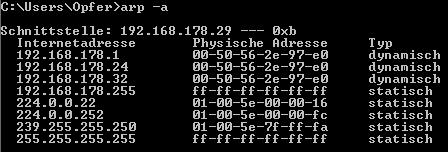
\includegraphics[width=\textwidth]{images/arp/ARP_Tabelle_Nachher}
	\caption{Manipulierte ARP-Tabelle des angegriffenen Rechners}
	\label{fig:arp_tabelle_nachher}
\end{figure}

Auch über das Sniffen des Netzwerkverkehrs lässt sich ARP-Spoofing erkennen, da der Angreifer in regelmäßigen Zeitabständen eine Menge ARP-Pakete aussenden muss. Dies muss nicht per Hand gemacht werden, da bereits Systeme existieren, welche den Netzwerkverkehr analysieren und z.B. die ARP-Replys prüfen. Dadurch können fehlerhafte und gefälschte ARP-Replys herausgefiltert und an den Benutzer gemeldet werden. Beispiele für solche Systeme sind Personal Firewalls von \emph{Sygate} oder \emph{SnoopNetCop Pro}.

\subsection{Angriff abwehren}
Um das ARP Spoofing zu verhindern, können statische ARP-Tabellen verwendet werden. Der Nachteil dabei ist, dass diese Tabellen dann nicht mehr dynamisch sind und sie für jeden Teilnehmer geändert werden müssen, wenn z.B. ein neuer Netzwerkteilnehmer hinzukommt.

Eine weitere Möglichkeit in Linux-Netzwerken ist, den Benutzern keine Root-Rechte zu verleihen. Da für das Senden von ARP-Replys diese benötigt werden, kann man so eine Manipulation unterbinden. Diese Möglichkeit bietet allerdings keinen Schutz vor Angreifern, die einen eigenen Rechner in das Netz einbringen oder einen Rechner mit einem Live Betriebssystem starten.
